\documentclass{fast-nuces-bs}

\usepackage{blindtext}
\usepackage{mathptmx}% Times Roman font
\usepackage[T1]{fontenc}
\usepackage{lipsum} 
\usepackage{sectsty}
\usepackage{tikz-uml}
\usepackage{titlesec}
\usepackage{adjustbox}
\usepackage{listings}
\usepackage{color}

\definecolor{codegreen}{rgb}{0,0.6,0}
\definecolor{codegray}{rgb}{0.5,0.5,0.5}
\definecolor{codepurple}{rgb}{0.58,0,0.82}
\definecolor{backcolour}{rgb}{0.95,0.95,0.92}

\lstdefinestyle{mystyle}{
	backgroundcolor=\color{backcolour},   
	commentstyle=\color{codegreen},
	keywordstyle=\color{magenta},
	numberstyle=\tiny\color{codegray},
	stringstyle=\color{codepurple},
	basicstyle=\footnotesize,
	breakatwhitespace=false,         
	breaklines=true,                 
	captionpos=b,                    
	keepspaces=true,                 
	numbers=left,                    
	numbersep=5pt,                  
	showspaces=false,                
	showstringspaces=false,
	showtabs=false,                  
	tabsize=2
}

\lstset{style=mystyle}

% Information about the Thesis 
% -----------------------------------------------------------------------------
% (All are compulsory, do not delete any line other than author Information)
% For e.g., usually there are 3 students in a group, so leave authorone, 
% authortwo, and authorthree, and delete authorfour.
%%%%%%%%%%%%%%%%%%%%%%%%%%%%%%%%%%%%%%%%%%%%%%%%%%%%%%%%%%%%%%%%%%%%%%%%%%%%%%%
\department{Department of Computer Science}
\faculty{Computer Science}
\degreeyear{2018}
\degreemonth{May}
\degreename{Computer Science}
\campuscity{Peshawar}
\authorone{Aziz Ullah}{p14-6111}
\authortwo{Najeeb Khan}{p14-6112}
\authorthree{Hafiz Saud Arshad}{p14-6097}
%\authorfour{John Cena}{p15-6789}
\supervisor{Dr. Omar Usman Khan}
\sessionduration{2014-2018}
\cosupervisor{Dr. Mohammad Nauman}
\deanname{Dr. Hasina Khatoon}
\directorname{Dr. Tariq Khan}
\hodname{Dr. Omar Usman Khan}
\fypcoordinatorname{Shakir Ullah}
\title{Real Time Pakistani Sign Language
	Recognition Using Kinect}
%%%%%%%%%%%%%%%%%%%%%%%%%%%%%%%%%%%%%%%%%%%%%%%%%%%%%%%%%%%%%%%%%%%%%%%%%%%%%%%

%%%%%%%%%%%%%%%%%%%%%%%%%%%%%%%%%%%%%%%%%%%%%%%%%%%%%%%%%%%%%%%%%%%%%%%%%%%%%%
% Former document starts below this
\begin{document}

\begin{acknowledgements}
	We are very thankful to Almighty Allah who is most Merciful and most Beneficent for
	giving us strength and courage to choose such challenging project and for completing it
	with great dignity and grace. Lots of people played a significant role in the completion of
	this project.
	We firstly thanks Dr. Omar Usman Khan who motivated us to select this project. He
	encouraged and showed us the way the project can be implemented. He has been very
	kind, supportive and patience to us since the beginning of our project. His guidance and
	experience brought us on the right track when we lost again and again.
	We are highly thankful to all of our teachers who had been guiding us throughout our
	project work. Their knowledge, guidance, and training enabled us to carry out this development work more efficiently. We would like to thank all our friends, colleagues and
	family for their support, motivation, and suggestions about the project.
\end{acknowledgements}

\begin{abstract}
We propose a system that would translate Pakistan Sign Language to text in real time.
As a prototype, the system is limited to recognition of four pre-defined sentences. The system takes
input from a Kinect Camera device as a person practices signs in front of it. The system
generates the sentences on the screen being practiced in the sign. Our 
system uses depth information right from the Kinect device and computes the time-series
of a sign being practiced. The system is trained on the four sentences using Random Forest. It  evaluates the input sign on the model established after training and displays the sentence
against the sign practiced on the screen as suggested (predicted) by model. Our tests report an accuracy of 85\% using this approach. Our work can
be extended to commercial scale based on the schema proposed by the project.
\end{abstract}

\chapter{Preliminaries and Introduction\label{sec:introduction}}
\section{Overview}
The Project title states "Real time Video based Pakistan Sign Language Recognition". Real time gives the sense that system will be producing output just as it is given an input i.e. very small time laps. Real time performance is one of the most demanded quality of a machine learning based software product. The video based approach means that we will be using multiple videos of signs for training (tuning) the model in order to use this model for purpose of prediction of an unseen example (practiced sign). The segment "Pakistan Sign Language" conveys that the signs that will be predicted by the system are of Pakistan Sign Language.  \\
The signer will be doing the sign in front of a Kinect Camera device. This is passed to the system. System evaluates the sign on model already built and outputs the text against the sign. Many such systems are developed and many more are in form of complete commercial products e.g. Motion Savvy and Microsoft Kinect Sign Language Recognition. This product does not intend to challenge the previous work rather this is an attempt to expand the cloud of this technology to Pakistan Sign Language Recognition.


\section{Motivation}
Around 360 million people around the world (5\% of world’s population) are suffering from some kind of hearing loss and many are those who cannot speak. This creates a sub-conscious barrier between such disabled persons and rest of the society. Such subjects use Sign languages to communicate. Many countries have developed technologies that could help such participants remove this barrier in order to get a healthy and transparent society. But sadly there’s been very little work done in Pakistan Sign Language (PSL) technologies. PSL Recognition systems created till now are limited to numbers and other signs like directions, colors and body parts etc. Most of PSL technologies are static sign language recognition. \\
System proposed is a dynamic sign language recognition technology that takes live video of PSL signs and predicts its meanings in textual form. This can contribute in flourishing of PSL and disabled people. 


\section{ Objective}
The objective of this project is to come up with a technology that takes visual input (live video) of a sign being practiced in Pakistan Sign Language and predicts what it means in textual form.


\section{ Target Group}
The intended subjects of this technology are the people who suffer from any kind of hearing loss and knows Pakistan Sign Language and those who want to communicate to a mute person and do not know Pakistan Sign Language.

\section{ Problem Statement}
Hearing impaired or mute people are cornered due to inability of communication with other people. Currently in Pakistan, there is no technology that could help them with communication. There is work done on this technology but that is only limited to static sign inputs. There is needed a system that works on dynamic inputs and could serve the purpose of Sign to text translation in real time.

\section{Solution proposed}
A video based machine learning approach is proposed that takes in video in real time and predicts the text against a sign practiced in video. This system can be trained on some pre-specified set of signs and a model for classification is established. Later a sign video can be evaluated on this model and classified accordingly.
\subsection{Motivation to use Kinect device for SLR}
The conjunction of depth map and color image from Kinect sensor could produce great contribution for sign language recognition in three aspects. First, with the depth map, back-ground modeling becomes more simple and robust. We can easily and accurately extract human body part from color images. Second, in previous 2-D solutions, how to track hands is a difficult task. However, the skeleton information, developed from depth map, can be utilized to locate the positions of hands robustly and in real time. Third, beyond the traditional 2-D features, Kinect senor can provide some novel 3-D features, which are quite useful and hence and improve the performance of sign language recognition. These advantages will emerge in our following experimental results.
\subsection{Motivation to use features from hand finger and skeleton}
These actually gives a visualization of how a hand performs a sign in physical and how an interpreter can interpret it. As a finger is bent, its distance from the successive finger changes, angle of the defect (joint) is also effected and the distance between the joint and a hull around the hand also changes. So a single moves provides uniqueness in all three dimensions of main features. This justifies that these features would be good to be used for unique pattern identification. 


\begin{figure}[!htb]
	\begin{center}
		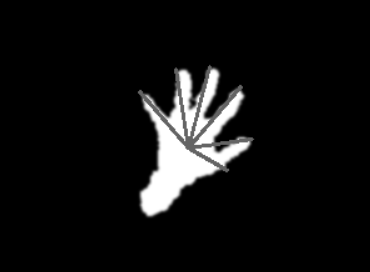
\includegraphics{ThesisFigs/skeletnon}
		\caption{Skeletnon of Hand }\label{fig:Skeletnon of Hand}
	\end{center}
\end{figure}


\subsection{Motivation to use Random Forest Classifier}
Random forest is actually an ensemble based learning in which we used multiple classifiers each a decision tree, and then predict the sign using all those trees. In the end, we assign probabilities to each class as with the ratio of predicted by trees and lastly we pick it based on the probability.
Moreover, our data is non-categorical or numeric (ordinal). Random works really well when the features are known. For each of the tree, it would apply multiple splits based on minimum entropy and maximum information gain.
Do in this case, Prediction is simpler i.e. just parse through the tree and predict the leaf class. Prediction does not take too much time. Prediction is ensemble so not a much chances to over fit on some class.

\section{Scope:}
This project can be installed to different scope domains like in hospital for training, communication and prescriptions. Following scenarios can use a furnished and modified form of this project.
\begin{itemize}
\item[•]\textbf{	Training:}\newline
There are patients in the hospital who have partial disability to speak, they use a bit of sign language to communicate. Such people can use the product. Also there are others who are deaf but they need to be trained how to speak i.e. how to twist the tongue, clump the lips and direct your voice. So they can be trained and communicated using this sign language machine by an ordinary person who does not know sign language. Moreover there are others who are complete deaf or mute, they also use sign language. For each of the above case, different sets of sentences could be selected for communication and make a custom model and use it.


	

\item[•]\textbf{	Communication with doctor:}\newline 
A doctor who does not know sign language can be made able to understand the problems of the mute patient. We can also enable the doctor to do the prescription to a deaf person using this machine by adding feature to replace the words with sign itself.
\end{itemize}
\section{Some related famous products: }
Following are the examples of already available state of the art products that are available to general public. Their technology in some aspects to the technology of the concerned project.
\begin{itemize}
	\item DICTA sign  \cite{DICTAsign}
	\item Motion Savvy  \cite{MotionSavvy}
	\item MS Sign Language Translator \cite{MSSignLanguageTranslator}
\end{itemize}


\section{	SWOT Analysis }

\begin{center}
	\begin{tabular}{ |p{7cm}|p{7cm}| } 
		\hline
		\textbf{Strengths} & \textbf{Weaknesses}\\
		\hline
		\textbf{Performance :} 
		Now a days, performance is main concern. System under consideration performs well in a constrained environment as specified in weaknesses. \newline 
		\textbf{Time:} \newline 
		This system works in real time so no more time lapses.\newline 
		\textbf{Reliability:} \newline
		Reliability is the best a promise a product can make to its users. The system assures reliability by assuring all software development measures and steps. \newline
		\textbf{Luminance: }\newline 
		Almost all other systems serving the purpose are confined by luminance i.e. proper lightning is necessary for system to work properly. Which is not the case with the system being proposed.
		& \textbf{Supplements:} \newline
		A Kinect Camera device is needed in order to get input as no ordinary camera can serve the purpose of depth frame capturing.  \newline
		\textbf{Portability:}\newline
		A laptop is enough to get the system working but it needs a Kinect Camera to be available also. Which is not an every place utility so needed to be carried along. More else the system is going to need to be configured before use. Not an instant plug and play module.\newline
		\textbf{Distance:} \newline
		The system works only when the sign is being practiced at a constrained distance of \# ft. Else way, the sign goes undetected and hence can’t be processed. \\
	
		\hline
		\textbf{Opportunities} &  \textbf{ Threats:}\\
		
		 \hline 
		 open source software is easily available to edit and extend. Their debugging is also easy, as it is open source so many people can extend it for their purposes and can debug. &
		  System pose no physical or social threats to anybody. It will only benefit those who use it. But yes, in a way, this may prevent someone to learn PSL by themselves  \\
		\hline
	\end{tabular}
\end{center}




\chapter{Review of Literature\label{ch:lit-review}}
There can be many techniques and approaches to address a problem. Many solutions can be developed to solve a single a problem. We studied a bunch of different approaches in the literature of SLR and analyzed them so that to study what benefit an approach over another. These approaches involved sub-unit based approach to extract hands from background, static gabor filter based approach to background subtraction, ESF descriptor approach to extract features and many more. A few of the major approaches that helped us to get a deeper insight and derive a strategy are given in below sections.

\section{Sub-unit based approach}
 This is a sub-unit based Sign language recognition culminating in a real time Kinect demonstration system. This approach uses different types of sub-units e.g. Location, Motion and Hand-shape sub-units tracked and identified by both 2D and 3D tracking data. These sub-units are then combined using a sign level classifier. Further two approaches are used for time-series processing. First is Markov Models (in form of DTW i.e. Dynamic Time Warping) to encode temporal changes in sub-units. Second is uses Sequential Pattern Boosting to apply discriminative feature selection at the same time as encoding temporal information. This approach is more robust and performs well in signer independent tests and improves accuracy from 54\% to 76\% and then to 85.1\% for signer independent tests. \cite{no1}


\begin{figure}[!htb]
	
	\minipage{0.9\textwidth}
	\caption{Sub-Unit Based Approach }\label{fig:image1}
	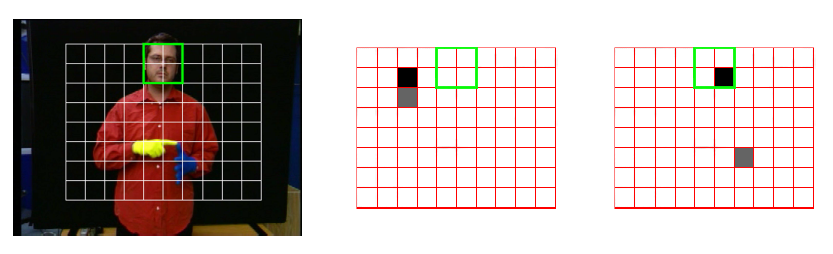
\includegraphics[height=3.4cm, width=15cm]{ThesisFigs/image1.png}
	
	\centering (a) Location based sub-units 
	
	\endminipage\hfill
	\minipage{0.4\textwidth}
	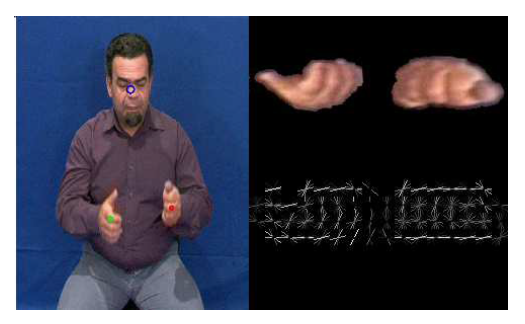
\includegraphics[height=3.2cm, width=\linewidth]{ThesisFigs/image2.png}
	(b) HOG Hand Shape descriptor
	\endminipage\hfill
	\minipage{0.4\textwidth}
	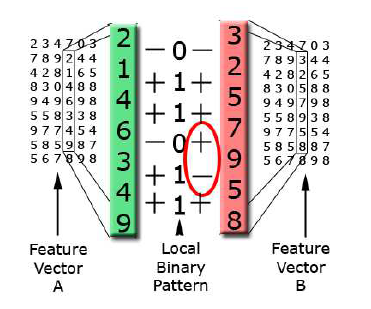
\includegraphics[height=3.2cm,width=\linewidth]{ThesisFigs/image3.png}
	(c) LBP Motion based descriptors 
	\endminipage\hfill
	
\end{figure}


\section{Static Gabor filter based approach}
 In this Research, Kinect Camera was used for input purposes keeping in mind that in this case input were images of static signs. Hand was segmented based on depth information right from the Kinect. Then hand shape features used are based on Gabor filtering of intensity and depth images. The purpose of using Gabor filter was that Gabor filter is apt at capturing contrast on image patch at different scales. Lately Random Forest was used for training and classification purposes on feature values obtained by Gabor filtering. A mean precision of 75\% was obtained following the considered approach.\cite{no2}

\section{ESF descriptors}
 Another approach used in previous computer scientists used ESF descriptors to unique identify different signs (static images). They used ToF (Time of Flight) cameras but techniques works perfectly fine with Kinect inputs just needs to be configured accordingly. ESF features were extracted from training samples and then trained with MLRF (Multi layered Random Forest). This is a simple approach which sacrifices accuracy for quick results. An accuracy of 85\% was observed practicing this approach.\cite{no3}

\section{Skin Intensity based hand-feature extraction}
 This approach proposes a technique that first takes intensity of skin color of sign and then segment the face, hand and elbow based on these intensity values. There are water-marks on the interface. In the few starting frames, signer has to place his elbow and hands on the specified water-marks. With these frames, algorithm is capable of finding the range of intensities of skin pixels. Then segment each of the frame to get the hand, elbow and face-region. The flatness of hand-region, CG of hand w.r.t face, area of hand, the direction of hand motion (depicted in below diagram) and the direction of hand-region by elbow angle.\cite{no4}


\begin{figure}[!htb]
	\begin{center}
		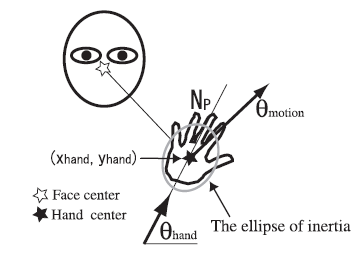
\includegraphics[height=4cm, width=8cm]{ThesisFigs/image0}
		\caption{Skin Intensity based hand-feature extraction}\label{fig:image0}
	\end{center}
	
\end{figure}

Feature set is fed to HMM (Hidden Markov Model).Which is used for prediction of signs.

\section{DTW based approach}
This approach is the most similar one to the project being presented; in this the whole words are being translated from sign videos not gestures. For this purpose, system takes the input from the Kinect as a series of frames. Then for all these frames, joints of interest are extracted which are the joints of two fingers in the ideal case. The distance between these joints and the Cartesian coordinates of the joints of interest (taking the origin at the center of the spine of signer’s body) are taken as features. As these features are extracted now a time series is built for the whole video. Later the time series is trained using the DTW. DTW matches the frames in the two (trained time-series and test time-series) and then predicts to the class with which it has lowest error. DTW on the backend uses an HMM. The most prominent feature of this pilot study was that the signs are taken from Pakistan Sign Language. \cite{no5}

\begin{figure}[!htb]
	\begin{center}
		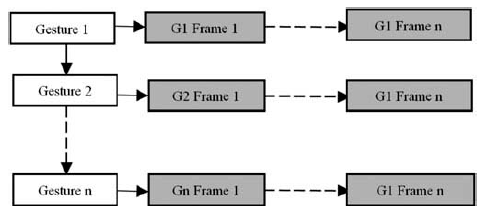
\includegraphics[height=5cm, width=12cm]{ThesisFigs/differentgesture}
		\caption{Different Gesture Format}\label{fig:Different Gesture}
	\end{center}
\end{figure}
The following picture demonstrates the dataset shape and organization






\chapter{System Analysis and Design\label{ch:System Analysis and Design}}

\section{Use Case}
\begin{tikzpicture}  

\begin{umlsystem}[x=0, fill=red!8]{Real Time Pakistani Sign language Recognition Using Kinect} 


\umlusecase[y=-1]{Get a Sign}  \umlusecase[y=-3]{Translate the Sign}  
\umlusecase[y=-5]{Record the sign}   \end{umlsystem}   

\umlactor[x=-7.5,y=-3]{listener} \umlactor[x=7,y=-2]{kinect}  \umlactor[x=7,y=-5]{Storage}   


\umlassoc{listener}{usecase-1}  \umlassoc{listener}{usecase-1}  \umlassoc{kinect}{usecase-1}  \umlassoc{listener}{usecase-2} 

\umlassoc{Storage}{usecase-3}   

\umlassoc{listener}{usecase-3} 

\umlassoc{Storage}{usecase-3} 

\end{tikzpicture}

Where the color spectrum from black to brighter gray represents the primary, secondary and outstanding actors
\clearpage
\section{Get the sign}
\begin{table}[htbp]
	\centering
	
	\caption{Get the Sign}
	
	\begin{tabular}{|p{3cm}|p{11cm}| } 
		\hline
		
		 Id &  1  \\ 
		\hline
		 Title &  Get Sign  \\ 
		\hline
		 Description &  Start getting the sign to be translated from the Kinect device.  \\ 
		\hline
		 Actor & Listener \\
		\hline
		 Pre-Condition & System must be 'On'.  \\ 
		\hline
		 Post Condition &  Frames of sign are being received live from Kinect Camera by the software. \\ 
		\hline
		 Success Scenario &  Learning module receives frames from the Kinect Device.  \\ 
		\hline
		 Alternative Flow &  Corresponding error displayed to user and program aborts.  \\ 
		\hline
		 Stakeholders &  Listener(operator), Signer.  \\ 
		\hline
	     Special Requirements &  Kinect must be powered, Kinect is successfully connected to the system.
		\\ 
		\hline
		 Open Issues &  The system when gets the sign then it stores the sign in an excel file. This file sometimes gets corrupted because of some internal file system error. \\ 
		\hline
	\end{tabular}  
	\clearpage        
\end{table}
A user arrives on the interface terminal. System presents him with three buttons labelled as ‘start’, ‘end’ and ‘Predict’. If user wants to get the sign recorded from the Kinect, he would press the ‘start’ button. The system has now started recording the sign. As the sign duration ends, the user has to press the ‘end’ button. As the ‘end’ button is pressed, sign is saved in the directory and can be used for further operations.

\clearpage
\subsection{Translate the sign}
\begin{table}[htbp]
	\centering
	
	\caption{Translate the sign}
	\begin{tabular}{ |p{3cm}|p{11cm}| } 
		\hline
		 Id &  2  \\ 
		\hline
		 Title &  Translate the sign  \\ 
		\hline
		 Description &  Sign is being received in form of series of frames from the Kinect Camera. Now this sign needs to be translated if Listener opts to translate.  \\ 
		\hline
		 Actor & Listener \\
		\hline
		 Pre-Condition & Program started receiving frames from the Kinect in form of series of frames.  \\ 
		\hline
		 Post Condition & Sign is evaluated and processed by the system and translated to a label or voice chunk. \\ 
		\hline
		 Success Scenario &  Sign is translated to a right label or voice chunk.  \\ 
		\hline
		 Alternative Flow &  Sign is translated to a wrong label or voice chunk.  \\ 
		\hline
		 Stakeholders &  Listener(operator).   \\ 
		\hline
		 Special Requirements &  Kinect must be powered, Kinect is successfully connected to the system,Sign must be recorded and stored successfully.  \\ 
		\hline
		 Open Issues & A naïve sign if done would be predicted to the class closest in features. So validity is only ensured if a sign is done from the predefined sentences. \\ 
		\hline
	\end{tabular}   
	
\end{table}
The signer has recorded the sign using the 'start' and 'end' button. Now he presses the 'predict' button. As he presses the button the system looks for the sign in the corresponding directory and then predicts it against the model. The 'label' is presented to the signer in the lower right text box. 

\clearpage
\subsection{Save the Sign}
\begin{table}[htbp]
	\centering
	\caption{Save the Sign}
	\begin{tabular}{ |p{3cm}|p{11cm}| } 
		\hline
		 Id &  3  \\ 
		\hline
		 Title &  Save the Sign  \\ 
		\hline
		 Description &  Sign can be saved to some repository and can be translated later if wanted.  \\ 
		\hline
		 Actor & Listener \\
		\hline
		 Pre-Condition & System must be 'On'.  \\ 
		\hline
		 Post Condition &  A sign is saved in form of a video to a repository. \\ 
		\hline
		 Success Scenario &  Sign was saved to repository.  \\ 
		\hline
		 Alternative Flow &  Corresponding error to user and system rolled back to previous safe point.  \\ 
		\hline
		 Stakeholders &  Listener(operator)  \\ 
		\hline
		 Special Requirements &  Kinect must be powered,
		Kinect is successfully connected to the system,
		All the libraries are successfully imported. \\ 
		\hline
		 Open Issues &  Note that only one sign can be saved for the future work not more than one.  \\ 
		\hline
	\end{tabular}   
	
\end{table}
The operator will record the sign using the 'start' and 'end' button. Now the operator presses the 'start' button
the data will be start storing when the operator clicks on 'end' button, the storage of the sign will be stopped.   

\clearpage
\section{Flow Diagram}
\begin{figure}[!h]
	\begin{center}
		
		\tikzstyle{decision} = [diamond, draw, fill=blue!20, 
		text width=4.5em, text badly centered, node distance=3cm, inner sep=0pt]
		\tikzstyle{block} = [rectangle, draw, fill=blue!20, 
		text width=6em, text centered, rounded corners, minimum height=4em]
		\tikzstyle{line} = [draw, -latex']
		\tikzstyle{cloud} = [draw, ellipse,fill=red!20, node distance=3cm,
		minimum height=2em]
		
		\begin{tikzpicture}[node distance = 3cm, auto]
		% Place nodes
		
		\node [block] (init) {Input Sign};
		
		\node [block, below of=init] (identify) {Segmentation };
		
		\node [block, below of=identify] (evaluate) {Time Series \\ Feature};
		
		\node [block, left of=evaluate, node distance=5cm] (update) {Time Series \\ Generation};
		
		\node [decision, below of=evaluate] (decide) {Model};
		
		\node [block, below of=decide, node distance=3.5cm] (stop) {Sign Label};
		
		
		\node [block, above of=update] (system2) {Feature \\ Extraction};
		
		\node [block, above of=system2] (system3) {Input Sign};    
		
		
		
		% Draw edges
		\path [line] (init) -- (identify);
		
		
		\path [line] (identify) -- (evaluate);
		\path [line] (evaluate) -- node {Testing} (decide);
		
		\path [line] (system3) -- (system2);
		
		\path [line] (system2) -- (update);
		
		\path [line] (update) |- node [near start] {Training} (decide);
		
		\path [line] (decide) -- (stop);
		
		
		\end{tikzpicture}
		
	\end{center}
\end{figure}



\clearpage
\section{System Sequence Diagram}

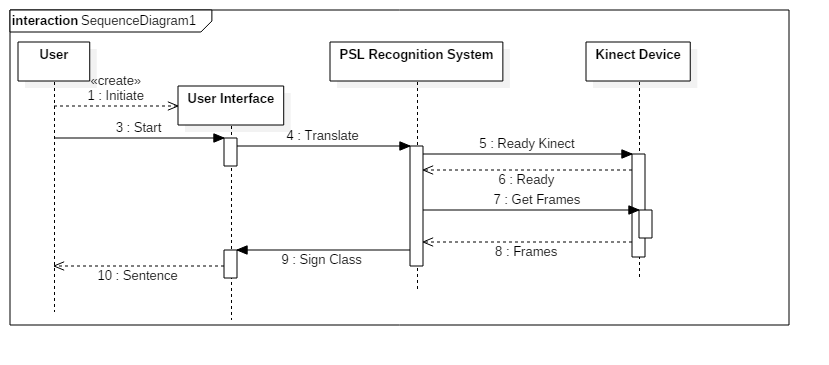
\includegraphics[height=10cm, width=17cm]{ThesisFigs/sequencediagram}


\chapter{Dataset\label{ch:Dataset}}
\section{Dimensions and Size }
In this section, we will explore the size and dimension of the dataset. How it is stored in the storage. Moreover, we are going to know, how dataset is built. How many instances are there? What does an instance look like? And much more.
\subsection{ Size: }
The dataset consists of 4 sentences (initially) to reflect the working and performance of the system being developed. The four sentences of Urdu are:
\begin{enumerate}
  \item Khush-Aamdeed.
  \item Ap kese hain ?
  \item Apka naam kia hai ? 
  \item Allah Hafiz 
\end{enumerate}

So dataset contains samples from each sentence. To create a balanced dataset, we’ve taken 22 instances of each class (sentence). Each instance is a video of sign being performed in front of Kinect camera. Each video is stored in form of an Excel file with each record representing a frame of the video. Length of videos is variable i.e. a sign may long 2 seconds and some other may long for 3 seconds. For a class, there may also be variable video lengths. Each file consists a number of rows representing frames in the video.
\subsection{ Basic unit }
Each video contains 'N' number of frames. 'N' varies from video to video and further varies from sign to sign. Each frame record contains 'M' number of features from the corresponding frame. These features of frames are the basic units of which an instance is composed of. 'M' varies from frame to frame. All the features from the frames of the videos are numeric and quantifiable.

\section{ Analysis: }
In this section, we will analyze the significance of dataset for building some model. We will see how well the dataset instances generalize a sign? How missing data occurs? What potential effects it can pose to the machine learning? How missing values are handled? All this analysis will be done in the following section.
\subsection{ Generalization }
For the generalization purpose, we've taken the signs from 3 different signers so that system does not over fits a single person. Each signer has performed 8 signs. Moreover, the video length is also variable that introduces some degree of generalization to dataset.
\subsection{ Missing Values }
As discussed, the feature length for a frame is variable. So for a file, there are frames stacked to each other in the xlsx file. So for a feature 'X' in a feature vector of frame 'A', 'X' may not be present in another frame 'B' causing a missing value (NA). Our dataset in contains a bundle of missing values and dataset is very noisy. Moreover, due to the variance in the length of the feature vector, it becomes very difficult to handle and use this data to make a model due to difficulty in data imputation.
\begin{figure}[!htb]
  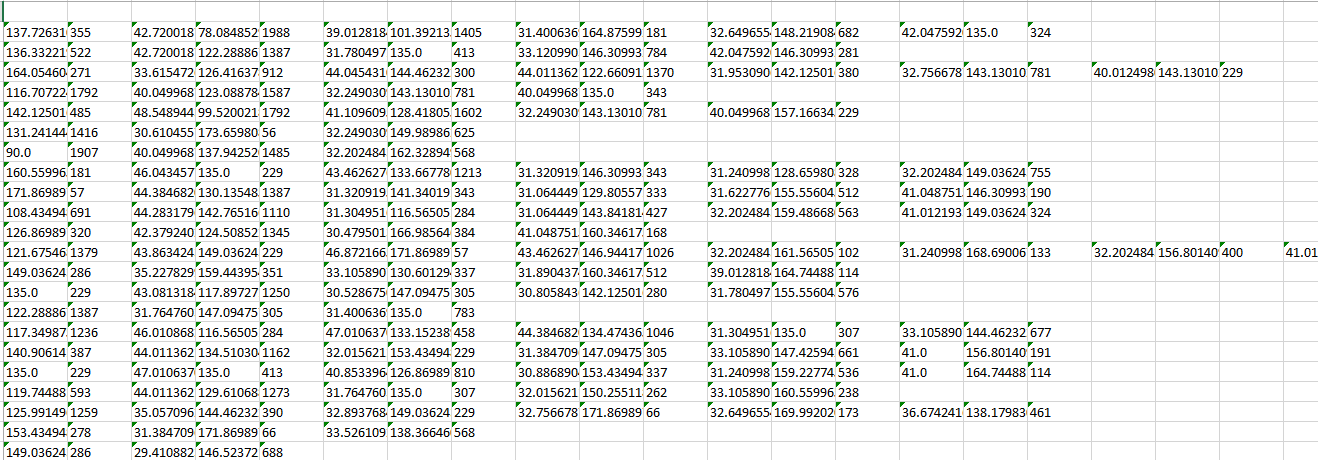
\includegraphics[height=6cm,width=15cm]{ThesisFigs/dataset1}
  \caption{Missing values in Dastsets }\label{fig:dataset1}
\end{figure}
\newline Above figure shows the missing values in as blank records.
\clearpage
\subsection{ Missing Records }
As video length is variable, so a video 'A' may have 'N' number of frames and another video 'B' may have 'P' number of frames. The difference between 'P' and 'N' is the missing frames length in the corresponding video.
\begin{figure}[!htb]
  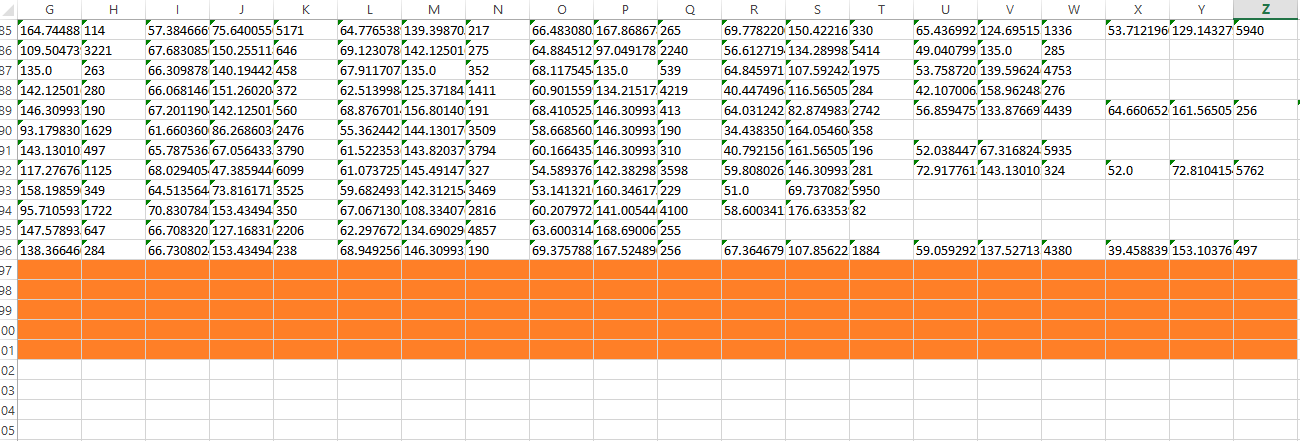
\includegraphics[height=6cm,width=15cm]{ThesisFigs/dataset2}
  \caption{Missing records in Dastsets }\label{fig:dataset2}
\end{figure}
\section{ Padding}
In order to do machine learning on the dataset we need each instance to be in the same shape and size. To achieve this purpose, we pad our data instances with zero.
\subsection{ Feature Padding }
We first find the maximum length feature vector. Then we pad each of the record with length less than the maximum length with zero to make compatible to the maximum length feature.
\subsection{ Frame padding}
And lastly, we pad each video with zero vectors so that to make it equal to the length of maximum length video.

\chapter{PROJECT IMPLEMENTATION\label{ch:PROJECT IMPLEMENTATION}}
\section{ Flow Diagram }
\begin{figure}[!h]
\begin{center}

\tikzstyle{decision} = [diamond, draw, fill=blue!20, 
    text width=4em, text badly centered, node distance=3cm, inner sep=0pt]
\tikzstyle{block} = [rectangle, draw, fill=blue!20, 
    text width=6em, text centered, rounded corners, minimum height=4em]
\tikzstyle{line} = [draw, -latex']
\tikzstyle{cloud} = [draw, ellipse,fill=red!20, node distance=3cm,
    minimum height=2em]

\begin{tikzpicture}[node distance = 4cm, auto]
    % Place nodes
      
    
     \node [block] (node1) {Kinect Input};
     
     \node [block,right of=node1] (node2) {Segmentation};
     
     \node [block,right of=node2] (node3) {Skeletonization};
     
     \node [block,below of=node3] (node4) {Feature \\ Extraction};
     
     \node [block,below of=node2] (node5) {Training \\  the Model};
     
     \node [block,  below of=node1] (node6) {Test a Sign};
     
    % Draw edges
  
    \path [line] (node1) |- (node2);
    
    \path [line] (node2) |- (node3);
    
    \path [line] (node3) -- (node4);
    
    \path [line] (node4) -- (node5);
    
    \path [line] (node5) -- (node6);
    %\path [line] (node5) |- node {ceja} (node6);
    
\end{tikzpicture}
    
\end{center}
\end{figure}

\section{Implementation}
We take input from Kinect using the python library pykinect. We capture the depth frame from the event handler depth frame. This depth frame tells us the different to the object in each pixel. This distance is a 16-bit value out of which one bit is redundant and 3 bits are for player index. So each distance is a 12-bit value. 
\hfill \break
This 12-bit frame is then normalized to 8-bits by bit-by-bit shifting. This 8 bit frame can be seen as an 8-bit image of gray scale. In which the nearer objects are darker than the far objects. So objects at minimum distance would be the darkest.

\begin{figure}[!htb]
	\begin{center}
		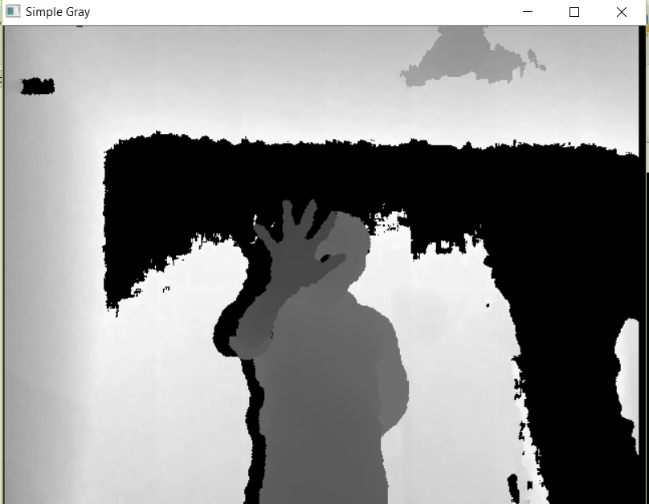
\includegraphics[height=6cm,width=8cm]{ThesisFigs/GrayImage}
		\caption{Gray Image Formation}\label{fig:GrayImage}
	\end{center}
\end{figure}
Note: Any object beyond the range of the Kinect’s optimum range is the darkest.
\hfill \break
Obtained 8-bit gray image is then segmented based on the minimum distance objects from the Kinect. Keep in mind that our project bears a constraint that the signing hand is the only object that is at the minimum distance from the Kinect. So by segmentation based on the minimum distance we get the hand region and using it as a threshold to binary image we will get a binary image with the only signing hand.
\begin{figure}[!htb]
	\begin{center}
		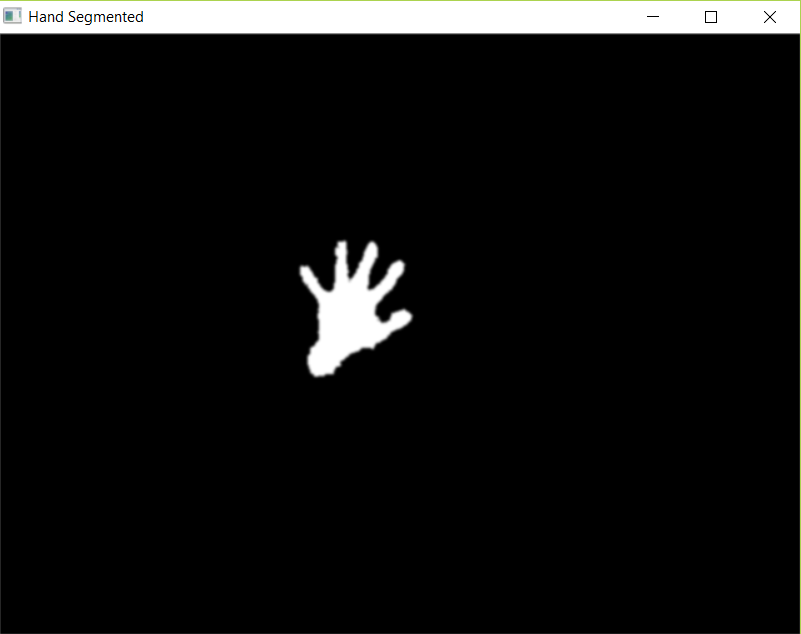
\includegraphics[height=6cm,width=8cm]{ThesisFigs/segmentedImage}
		\caption{Segmented Image}\label{fig:segmentedImage}
	\end{center}
\end{figure}
A segmented image of the above shown gray image is shown.
\hfill \break
We then need to identify all the fingers and the center of the so that these points could be used to generate the feature vectors. For that, we first find the contours (boundary) of the hand. We also find the convex hull in the of the hand shape. Now try and find the points that are common to both the convex hull and the contour of the hand. Both the Convex hull and contours are extracted using OpenCV python. These are the points to be identified as finger tips and corners of the hand. Finger are identified and now these can be used to extract features.
\begin{figure}[!htb]
	\begin{center}
		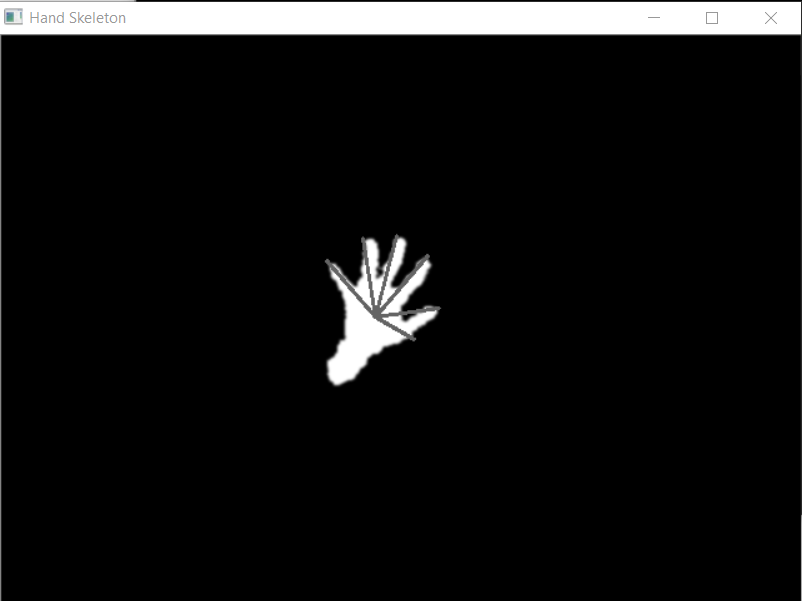
\includegraphics[height=6cm,width=8cm]{ThesisFigs/skeletonImage}
		\caption{Skeleton Image}\label{fig:skeletonImage}
	\end{center}
\end{figure}
Now we find the sum of x-coordinates and also the sum of y-coordinate of all the white pixels (hand-region). Now we divide both x-sum and y-sum by the total number of hand pixels. The obtained point i.e. (x, y) pair is the centroid of the hand.
\hfill \break
Knowing all the main points of the hand region in the frame, we now extract features from the frame to make a feature vector. There are following four main features used:

\begin{itemize}


   \item[•] \textbf {	Consecutive fingers gap :  \\}
  We take the gap of the two consecutive fingers (our choice whether counting from left to right or right to left). This gap      is calculated in the following way:
Say the two fingertips were ‘A’ and ‘B’ points.


\begin{align}
&\sqrt{ [( A.x - B.x )^2 + ( A.y - B.y )^2]} = Distance value (number of pixels)
\end{align}
\item[•] \textbf { Angles of the defects : \\}
  By using the convexity defects (extracted by convex hull and contour of the hand), we get to find the deepest point of the defect which is the considered to be the joint between the two fingers. Now for two consecutive finger tips ‘A’ and ‘B’, we form two vector:
  \begin{enumerate}
  \item From the fingertip ‘A’ to the middle joint of ‘A’ and ‘B’. 
  \item From the fingertip ‘B’ to the middle joint of ‘A’ and ‘B’.
  \end{enumerate}
  Now for the two tips ‘A’ and ‘B’, we get vectors say ‘a’ and ‘b’. Now we apply the following formula.
\begin{equation}
a.b=|a|.|b|cos\theta
\end{equation}
   
From here, if we find the magnitude of ‘a’ and ‘b’ using the distance formula from point ‘A’ to joint and point ‘B’ to joint. And finally, we get angle from the above formula. Now we do that for every defect and use these angles in the feature vector.
 \item[•] \textbf { Area of the hand  : \\}
Area of the hand is number of pixel in the hand region in the respective frame. 
 \item[•] \textbf {Normal distance to convex hull : \\}
Normal distance from each of the joint to the convex hull. The distance is calculate for number of unit pixel and using the simple distance formula.
\end{itemize}

We concatenate all these triplets and area of the hand to form the feature record for the frame. We do that for all the frames and then take them record by record and make a whole file where each record represents a frame in the video.
\\
We combine all these videos of signs and then place all same signs in the same directory and same for all the other classes. As presented in the previous portion (4.3), we pad each video to the length of the maximum size video so that each instance be of the same size and be feasible to train. For padding purpose, we use the Keras python. \\
As all the dataset is in its final form so let’s move in to build the machine learning model for the prediction of signs. A random forest was trained on this dataset with 50 number of trees each of depth 24. Class label was assigned based on majority votes of the tree. Dataset is partitioned to two sets of 75\% part of the whole dataset for training purpose and the rest 25\% part of the dataset for evaluation of the model. Sklearn in python is used to build the model.\\
The interface is built in tkinter python. It contains a window that shows the frame coming right from Kinect. Another field that present you with the label of sign being performed in front of the Kinect. There are also two more buttons labelled as ‘start’ and ‘Predict’. ‘Start’ serves the purpose to allow all the users perform the sign in front of the Kinect. And ‘Predict’ button can be used to terminate the sign duration. As the signer is done with his sign (presses the ‘predict’ button), the sign would be converted into the feature vector and evaluated against the model. In the result of evaluation, a label corresponding to the sign is extracted. This would be presented as the label (textual meaning of sign in Urdu) of the sign performed on the interface screen. \\
For prediction purpose, Random forest is used to classify the signs into sentences. Random forest is a simple but elegant ensemble machine learning technique. It is an ensemble of multiple simple machine learning classifier known as decision trees. It tries to predict class for the sign using different architecture trees i.e. different splits and bootstrapping on the train set. Then takes votes from these trees. And provides the results with majority votes.
As far as Decision trees are concerned, these are simple trees with each node of the tree is a split criteria for a feature. Splits are chosen based on maximum information gain and minimum entropy. And at the leaf there is the class label. An instance when parsed through this tree satisfying different split reaches to its class label. 

\clearpage
\section{Baseline Results}
As discussed and explained in the chapter-4, the complexity and noise of the dataset is huge. Moreover, to make it feasible, we padded the dataset; this also introduces some noise and bias in the dataset. Due to all those reasons, each frame carries some noise with itself and then later this noise convolves with noise of the whole video instance. Presence of all these noises in our dataset leads to a weak model. So the results (predictions) from this model are not fully reliable.\\

The accuracy achieved is 83\% as observed on the 25\% test dataset. Moreover, F1 measure is 0.83.
The prediction time taken by a system of following specification:

\begin{enumerate}
	\item[•]Intel Core i5 processor
	\item[•]8GB RAM
	\item[•]No GPU used
\end{enumerate}

Is 0.446 seconds approximately.
Note that these results are considered as running the system in offline mode i.e. not from the interface. While using the interface accuracy drops because of the frame closing and getting latency introduced by the operations of interface.
\clearpage

\section{Results}
The results are obtained using 10-cross-folds. The simple split across the dataset is 90\% for train and 10\% for test for each fold. Accuracy and F1 score are reliable and significant.\\


\textbf{Results using Random Forest classifiers}
\hfil \break
Results for all folds while using the Random Forest model are shown in Table \ref{randomforest}:

\begin{table}[h]
	\begin{adjustbox}{max width=\textwidth}
		\begin{tabular}{ |p{1.7cm}|c|c|c|c|c|c|c|c|c|c|} 
			\hline
			&  Fold-1 &  Fold-2 &  Fold-3&  Fold-4&  Fold-5&  Fold-6 &  Fold-7	 &  Fold-8&  Fold-9 &  Fold-10     \\ 
			\hline
			Accuracy &  91.667   &  91.667   &  91.667   &  83.333  &  58.333  &  83.333   &  75.0	 &  83.333  &  75.0    &  100.0 \\ 
			\hline
			F1-Score &  0.9144   &  0.9142 &  0.9142&  0.8035&  0.5761&  0.8309     &  0.7416	 &  0.8309&  0.7321 &  1.0 \\ 
			\hline
		\end{tabular}
	\end{adjustbox}
	\caption{Results using Random Forest classifiers\label{randomforest}}
\end{table}

 

The accumulated and finalized results obtained the above given technique and prediction using Random Forest are:

 Cumulative Accuracy of the dataset:	\quad\quad	0.825 (82.5\%) \\
Cumulative F1 Score of the dataset:	\quad\quad	0.83 \\
Entropy and Gini both were used as a splitting criterion and in the test many experiments were run using different number of trees as shown in the figure 5.4 below.
\begin{figure}[!htb]
	\begin{center}
		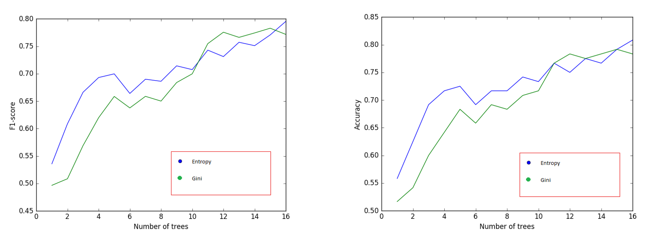
\includegraphics[height=6cm,width=14cm]{ThesisFigs/randomforestgraph}
		\caption{Random Forest Result Graph}\label{fig:randomforestgraph}
	\end{center}
\end{figure}


\clearpage

\textbf{ Alternative Results using SVM classifiers}
\hfil \break
Results for all folds while using the SVM model are shown in Table \ref{svm}:

\begin{table}[h]
	
\begin{adjustbox}{max width=\textwidth}
	\begin{tabular}{ |p{1.7cm}|c|c|c|c|c|c|c|c|c|c|} 
		\hline
		&  Fold-1 &  Fold-2 &  Fold-3&  Fold-4&  Fold-5&  Fold-6 &  Fold-7	 &  Fold-8&  Fold-9 &  Fold-10     \\ 
		\hline
		Accuracy &  100    &  83.333   &  66.6666   &  75  &  50  &  58.333  &  41.666	 &  66.6666  &  75.0    &  100.0 \\ 
		\hline
		F1-Score & 1.0 &	0.8333 &	0.675 &	0.7428 &	0.5	& 0.5863 &	0.3653	& 0.675	& 0.7321 &	1.0 \\ 
		\hline
	\end{tabular}
\end{adjustbox}
	\caption{Results using SVM classifiers\label{svm}}
\end{table}


The accumulated and finalized results obtained the above given technique and prediction using SVM are,

  Cumulative Accuracy of the dataset:	\quad\quad	0.71 (71\%) \\
 Cumulative F1 Score of the dataset:	\quad\quad	0.72 \\

Experiments were run using different degrees of the hyperbola separating the classes. Results are shown in diagram. 
\begin{figure}[!htb]
	\begin{center}
		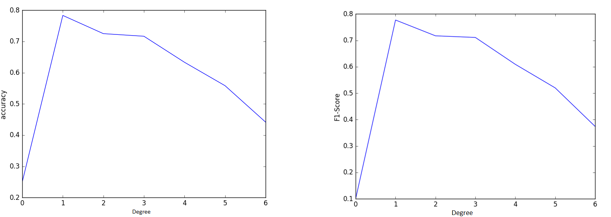
\includegraphics[height=5cm,width=14cm]{ThesisFigs/svmgraph}
		\caption{SVM Result Graph}\label{fig:svmgraph}
	\end{center}
\end{figure}




\textbf{	Alternative Results using Decision Tree classifiers}

\hfill \break Cumulative Accuracy of the dataset:	\quad\quad	0.53 (53\%) \\
  Cumulative F1 Score of the dataset:	\quad\quad	0.55 

Many splitting criterion used are entropy and gini with ranging the depth of tree. Results are shown by fig below. 
\clearpage
\begin{figure}[!htb]
	\begin{center}
		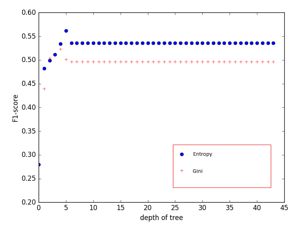
\includegraphics[height=7cm,width=12cm]{ThesisFigs/decisiontreegraph}
		\caption{Decision Tree Result Graph}\label{fig:decisiontreegraph}
	\end{center}
\end{figure}

\textbf{Alternative Results using Naïve Bayes classifiers}
\hfil \break
We also used Naïve Bayes to serve the purpose or build the model. Naïve Bayes worked also fairly well as shown by the following results.

Results for all folds while using the  Naïve Bayes model are shown in Table \ref{naviebayes}:
\begin{table}[h]
	
\begin{adjustbox}{max width=\textwidth}
	\begin{tabular}{ |p{1.7cm}|c|c|c|c|c|c|c|c|c|c|} 
		\hline
		&  Fold-1 &  Fold-2 &  Fold-3&  Fold-4&  Fold-5&  Fold-6 &  Fold-7	 &  Fold-8&  Fold-9 &  Fold-10     \\ 
		\hline
		Accuracy &  50  &	66.666	& 50	& 50	& 25	& 25	& 25	& 41.666	& 75.0	& 58.333\\ 
		\hline
		F1-Score & 0.502 &	0.675	& 0.521 &	0.475 &	0.182	& 171	& 0.214	& 0.375	& 0.555	& 0.497 \\ 
		\hline
	\end{tabular}
\end{adjustbox}

	\caption{Results using  Naïve Bayes classifiers\label{naviebayes}}
\end{table}

\hfil \break
 Cumulative Accuracy of the dataset:	\quad\quad	0.45 (45\%) \\
Cumulative F1 Score of the dataset:	\quad\quad	0.41 \\




\section{Alternative flows and approaches followed}
We tried many flows and strategies but at some point they collapsed or during the feasibility study, they were found to be not compatible with the problem statement. Following are the strategies as listed below.

\begin{enumerate}
	\item \textbf{ RGB and Depth-image overlap for segmentation }
In the starting few frames user is asked to keep his hands in the front of his body and at minimum distance from Kinect. Now take 'AND' of these pixels of binary segmented image with the pixels of the RGB frame to extract the hand region. And now find the bounding box of this hand region in the RGB frame. Extract this region and find its HOG features and append these HOG features from all frames of the video to make feature vector of the sign video.

\item[•] \textbf{Problems with the approach}
\begin{enumerate}
\item The depth frame is zoomed in as compared to the RGB frame. When over-lapping these region would also include some noise of the surrounding.
\item[•]To compute HOG feature, Image must be in the 8 or 16 bit-depth. So to do that, we have to convert each frame to Gray first and then compute HOG. Which takes quite much time; we may lose some key frames. This would take much time and may not allow us to predict in real time for a much larger dataset.
\item HOG features approach would be redundant because for this approach; an instance feature vector would be very huge.
\item[•]For Each frame; the segmented region would be different; we will have to pad the HOG frame to make the size of all frame equal.
\end{enumerate}


\item \textbf{Only RGB hand-tracking and feature Extraction\\}
We had done the hand tracking; our algorithm was tracking the hand with always changing hand shape for each successive frame. Tracking was Real time. Tracking was done using Dlib module that uses localized histograms to get features from a frame and then use these features to track the hand in the successive frames. HOG features were also extracted by converting each frame to gray.
\item[•] \textbf{Problems with the approach}
\begin{enumerate}
\item[•]The Kinect RGB camera is quite noisy. So the hand region that was observed by the specified region from first frames was itself noisy. So while defining the intensity range it would have considered the noise but that was handles by using only the region in the range of standard deviation. But then it starting also segmenting the face and neck region of intensity values. Same were the problems with segmentation based on HSV (Hue, Saturation and Lightness).
\item[•]Region filling in this region was a hectic and noisy job to do.
\item[•]After even segmentation, we were to use some features like HOG or SURF which were redundant in larger and bigger datasets.
\item[•]No significance to use the Kinect Device, if we are to use only the RGB frame.
\end{enumerate}

\item \textbf{Hu-Moments and Zu-Moments \\}
Hu- moments and Zu-Moment are state-of-the-art features to predict static objects and to check whether an object differs from others or not. They are rotation, position and scale invariant features that is why used in many of the applications. We did not extracted these from our frames because we found it these not worthy enough to serve the purpose in this project purpose.
\item[•] \textbf{Problems with this approach}
\begin{enumerate}
\item[•]In the sign language, there is a great significance of hand angle (if hand is rotated or not). As these features are rotation invariant so this would consider a tilted hand and a straight hand as same.
\item[•]These features are significant for only the case, when there are gray values in the region of interest (hand region) but when hand region is identified then it is all the same (flat) intensity values because there is no significant different in the distance from the Kinect Device.
\item[•] No significant results are extracted for sign recognition in the literature.
\end{enumerate}

\item \textbf{LBP features  \\}
LBP features approach finds the local binary patterns as suggested by the names. It goes across the whole image and finds the intensity shifts and captures those in a feature vector for a frame. These features were exempted during the feasibility study phase.
\item[•] \textbf{Problems with this approach}
\begin{enumerate}
\item[•]These features are significant for only the case, when there are gray values in the region of interest (hand region) but when hand region is identified then it is all the same (flat) intensity values because there is no significant different in the distance from the Kinect Device. So no gray region would be in the hand region and hence intensity shifts will remain undetected.
\item[•]No significant results are extracted for sign recognition in the literature.
\end{enumerate}

\item \textbf{SIFT and SURF features  \\}
SIFT as suggested by the name are Scale invariant features which is a plus point in our case. These features apply on RGB and Gray images.
\item[•] \textbf{Problems with the approach}
\begin{enumerate}
\item[•]To compute SURF and SIFT features, Image must be in the 8 or 16 bit-depth. So to do that, we have to convert each frame to Gray first and then compute features. Which takes quite much time; we may lose some key frames. This would take much time and may not allow us to predict in real time for a much larger dataset.
\item[•]SURF and SIFT features approach would be redundant because for this approach; an instance feature vector would be very huge.
\item[•]For Each frame; the segmented region would be different; we will have to pad the SIFT and SURF frame to make the size of all frame equal.
\end{enumerate}

\end{enumerate}
\clearpage
\section{Interface Description}
There are three blocks on the interface. The left block displays the depth stream (transformed to gray image) from the Kinect. The upper right block displays the segmented and skeletonized frame against the frame in the left block at the same time. And lastly, the lower right block contains four item.\\
\begin{itemize}
	\item[•] Text/Label window: Displays the output label against the sign perform in front of the Kinect.
	\item[•]	Start button: Allows user to start performing (recording) the sign.
	\item[•]	End button: Allows the user to stop performing the sign.
	\item[•]	Predict button: Once the sign is performed and saved using the ‘end’ button. User can predict this sign to sentence label using the ‘predict’ button.
\end{itemize}
An interface depiction is given below in which a sign is being performed.

\begin{figure}[!htb]
	\begin{center}
		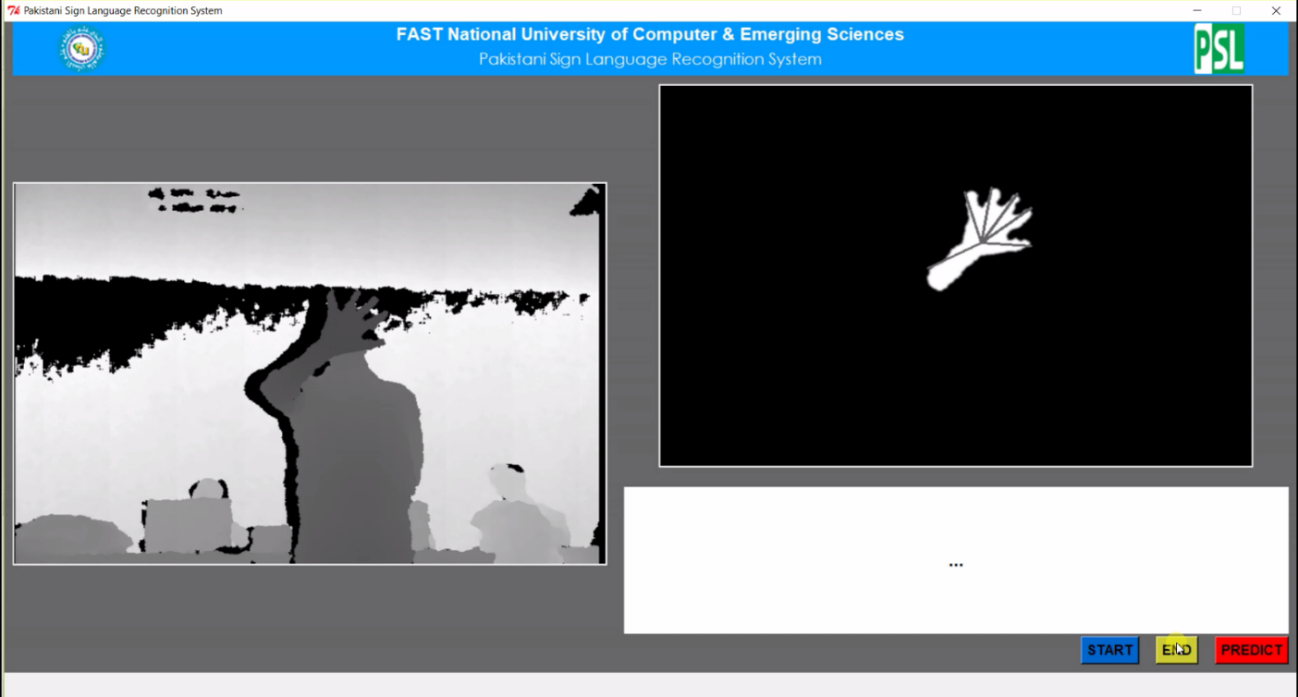
\includegraphics[height=8.5cm,width=12cm]{ThesisFigs/userinterface}
		\caption{User Interface}\label{fig:userinterface}
	\end{center}
\end{figure}
\clearpage
When you press the ‘predict’ button, the label or sentence against the sign is displayed in the Text/Label box as predicted by the model. As depicted by the following image.

\begin{figure}[!htb]
	\begin{center}
		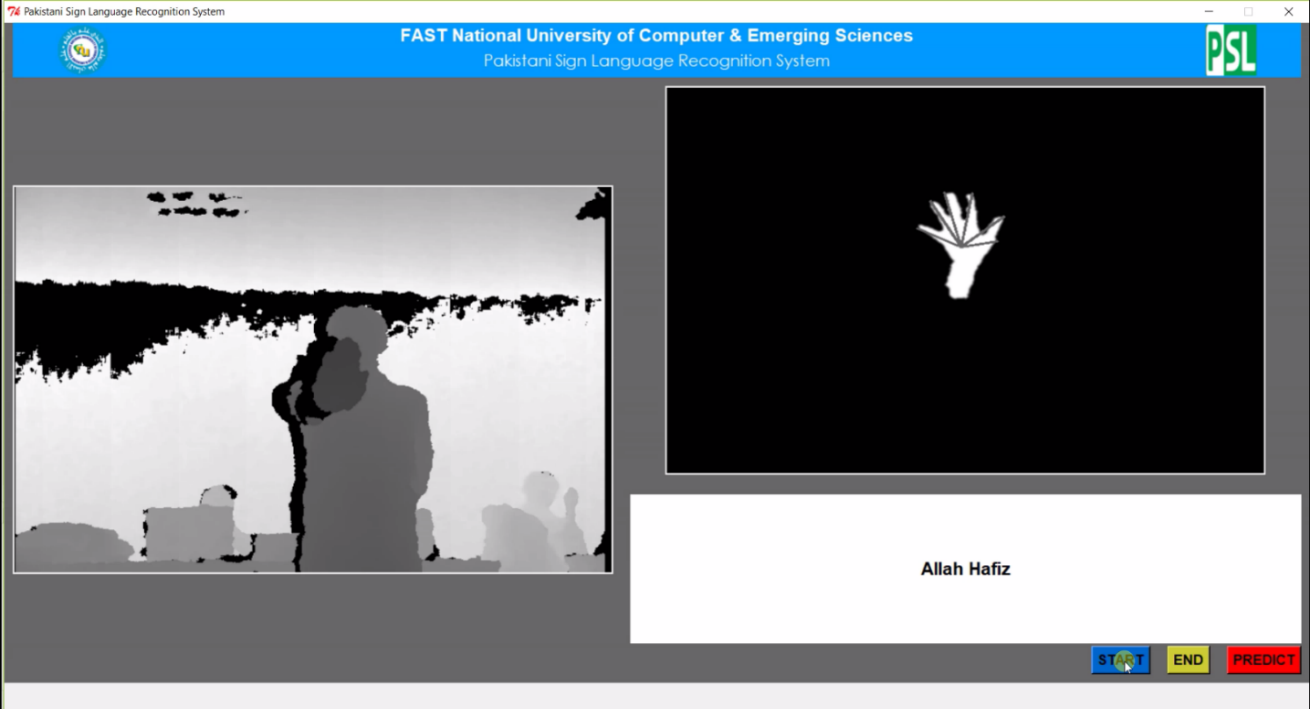
\includegraphics[height=8.5cm,width=12cm]{ThesisFigs/userinterface2}
	
	\end{center}
\end{figure}



\chapter{Future Recommendation}

This project is the minimum working example of a bigger, more universal and applied system that can be extensively used in many industry based and personal use application. This project serves the purpose in 4 sentences initially. Although the NLP problem is computationally infeasible, but if make an attempt to fit to some legitimate, small and limited scope application, we can cover most of the domain. \\

Currently system works for only single handed gesture. Develop a technique (most probably using RGB and Depth both) to segment both hands from the frame and then you can apply it universally to any sign.\\

Now we can extend this system by identifying a number of generally and frequently used sign language sentences. Prepare a dataset out of them by using at least two different signers. Feed into the system and retrain the model. Now attach (configure) this model to the prediction by configuring the file name and you are good to go. Use it in the environment.


\appendix
 \chapter{Appendix I Code}
 
\lstinputlisting[language=Python]{pakistani-sign-language-recognition.py}

 \chapter{Appendix I Poster}
 
\begin{figure}[!htb]
	
	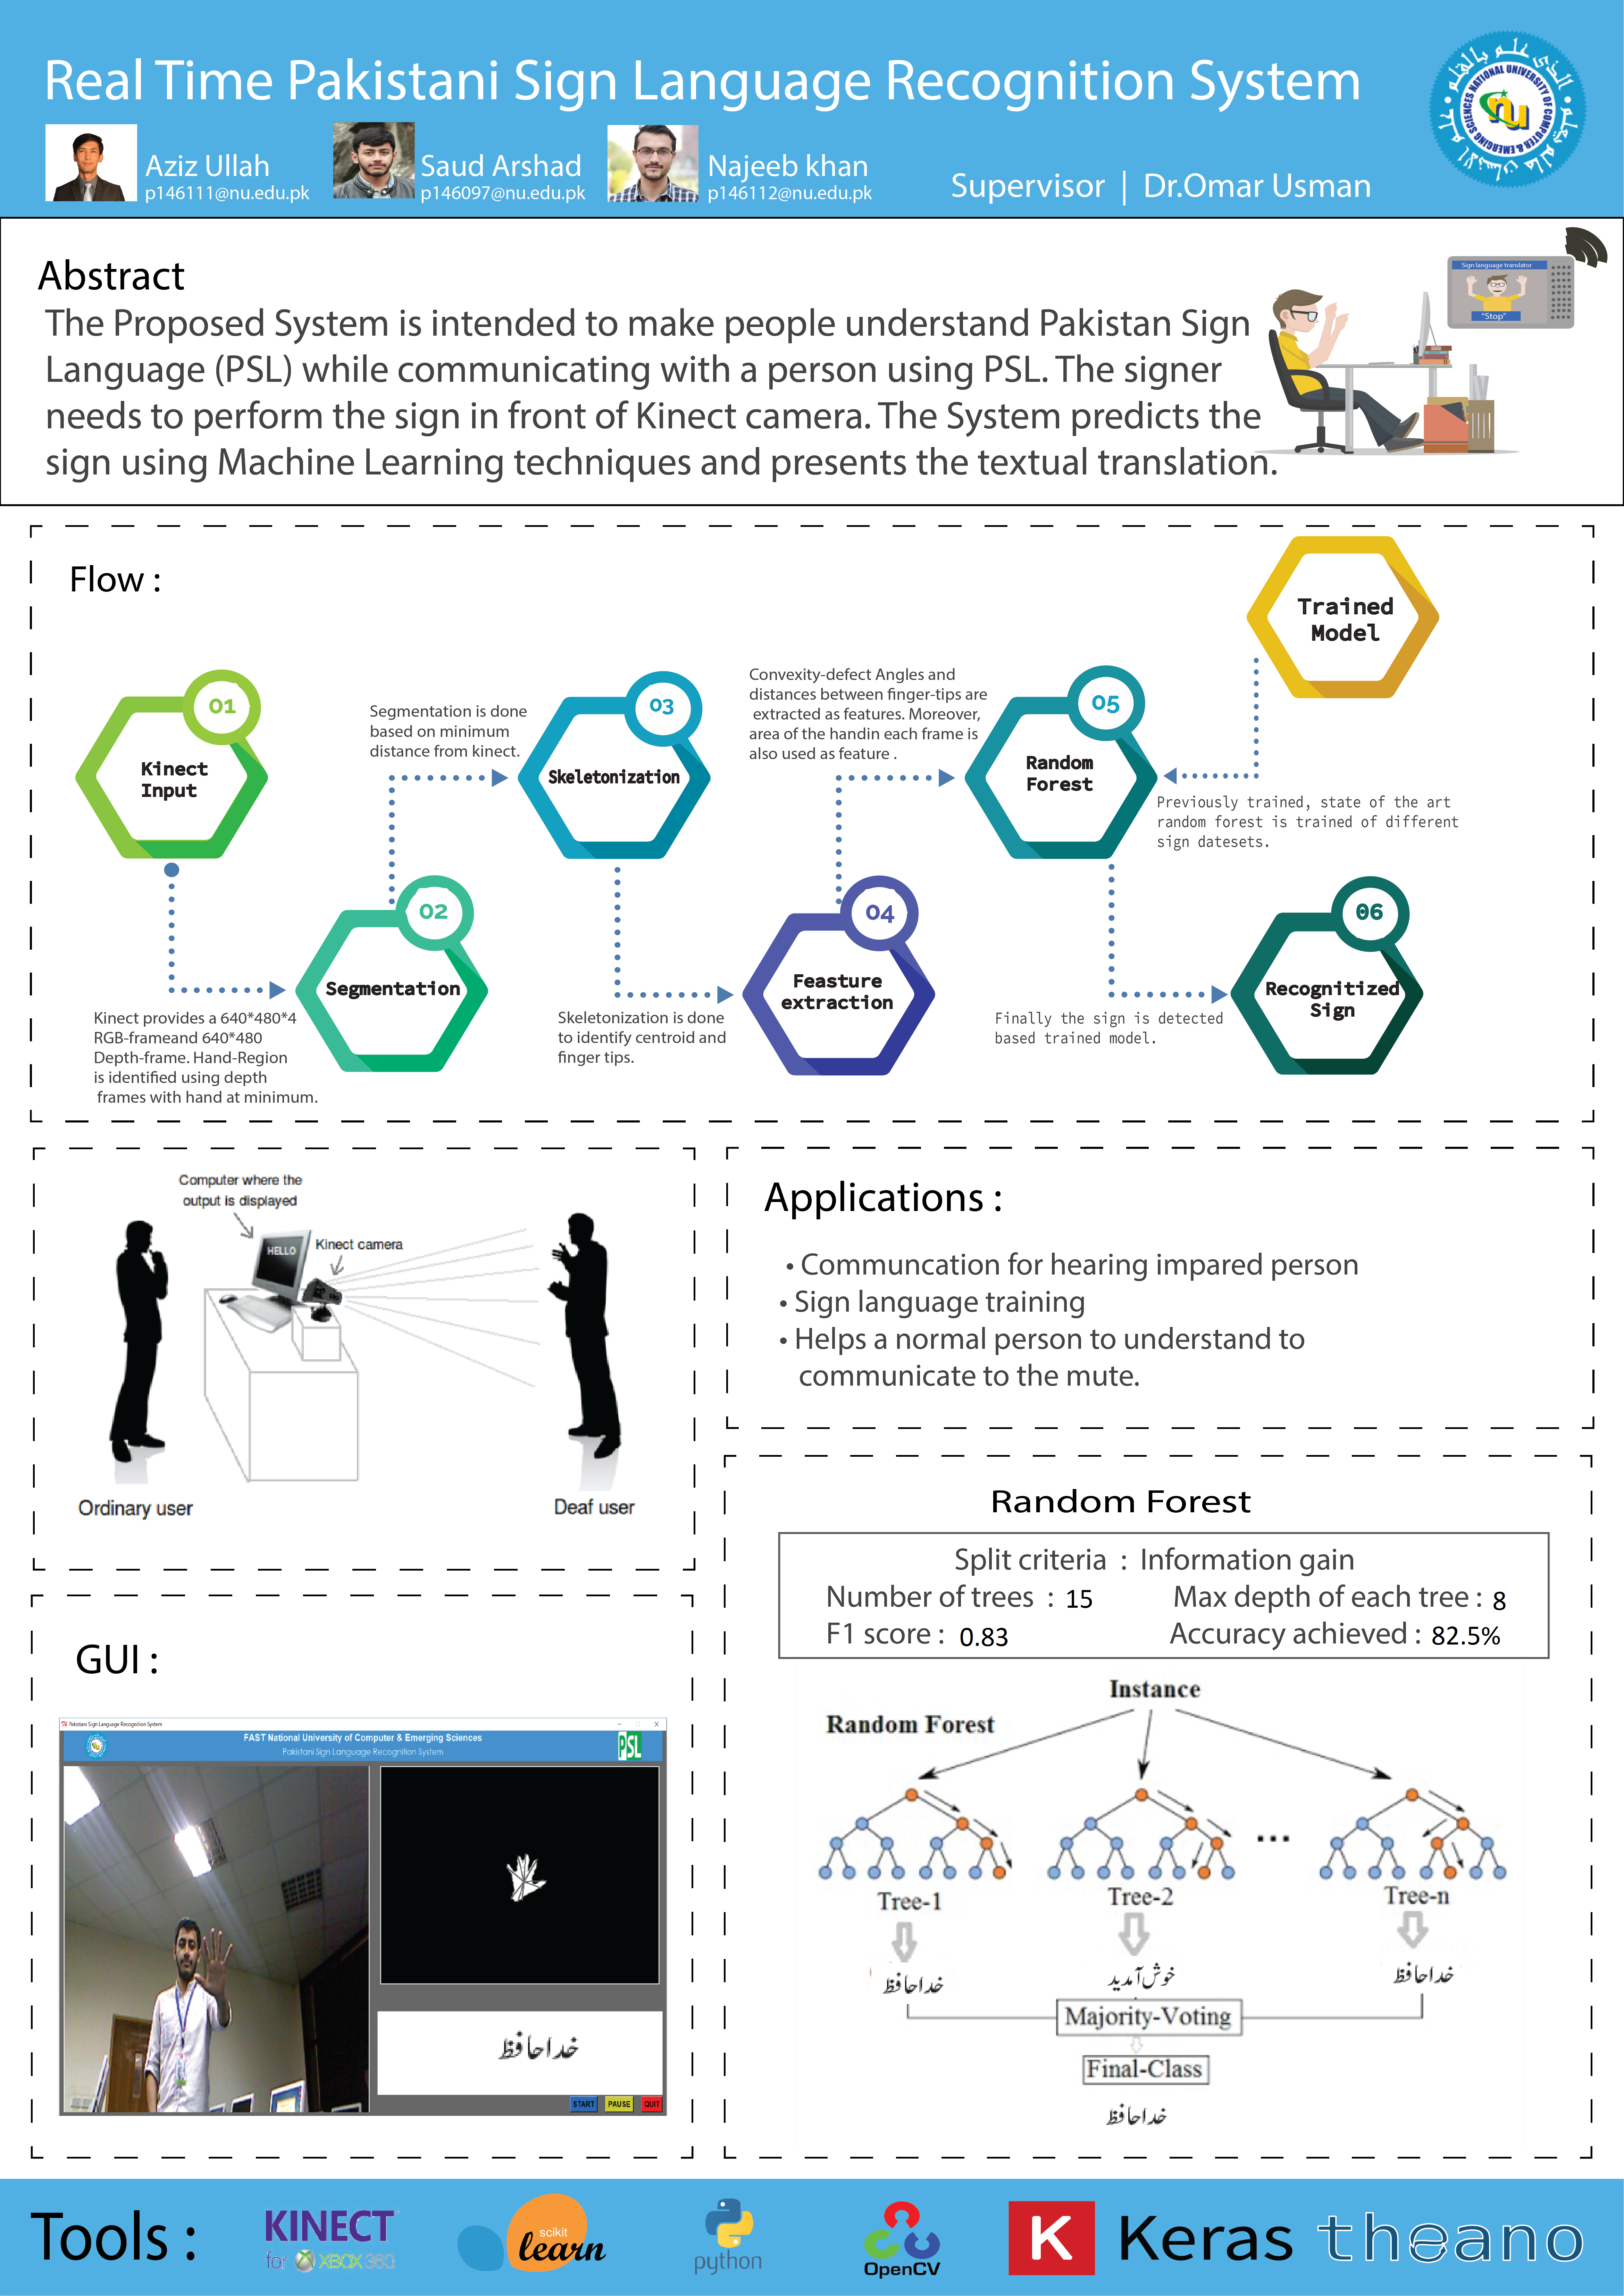
\includegraphics[width=1\columnwidth]{ThesisFigs/poster}
	\caption{Poster}\label{fig:poster}
\end{figure}


\bibliographystyle{plain}
\bibliography{bib} 
\addcontentsline{toc}{chapter}{References} 

\end{document}
